\section{Desarrollo de los puntos}

\subsection{Biohazard}
En primer lugar es necesario recordar brevemente de qué trataba el problema \emph{Biohazard}:
\begin{quotation}
  Una empresa de logística necesita transportar en camiones $n$ productos químicos desde una fábrica
  hacia un depósito seguro. Cualquier producto puede ser transportado en cualquiera de los camiones
  y para cada par de productos $p_i$ y $p_j$ se conoce de antemano el coeficiente de peligrosidad $h_{i,j}$
  que conlleva transportar dichos productos en el mismo camión. Los camiones tiene un umbral de peligrosidad
  que no puede ser superado. Respetando esta restricción se desea averigüar la mínima cantidad de camiones
  necesaria para transportar los productos.
\end{quotation}
Ambos problemas pertenecen a una clase de problemas conocida como optimización combinatoria. La misma
puede describirse rápidamente como la búsqueda de un objeto óptimo dentro de un conjunto finito de objetos,
donde el criterio de optimalidad está determinado por la maximización o la minimización de una función
específica. Una forma clara de describir un problema en particular de optimización combinatoria es
definiendo sus partes:
\begin{itemize}
  \item El espacio de soluciones $X$.
  \item El predicado de factibilidad $P$.
  \item El conjunto de soluciones factibles $Y$.
  \item $f$ la función objetivo que queremos maximizar o minimizar.
\end{itemize}

Comparemos las diferentes partes de los dos problemas:

\begin{center}
  \begin{tabular}{ >{\centering}m{1cm}<{\centering} | m{7cm} | m{7cm} }
      \centering Parte & \centering Biohazard & \centering $k$-PMP \tabularnewline \hline
      $X$ & 
      Tomando a los productos como elementos de un conjunto $C$ el espacio de soluciones consta de todas
      las particiones del conjunto $C$. & 
      El espacio de soluciones cuenta con todas las particiones de $V$ en un
      número de $k$ o menos conjuntos ya que puede haber particiones de nodos vacías.\tabularnewline \hline
      $P$ & La suma de las peligrosidades de cada una de las particiones no supera el umbral de peligrosidad de la instancia. & 
      En este caso el predicado factibilidad es siempre verdadero ya que cualquier partición en $k$ o menos subconjuntos
      puede ser la solución. \tabularnewline \hline
      $Y$ & Todos los elementos de $X$ que cumplan $P$. Todas las particiones que no tengan un camión con una peligrosidad mayor al umbral permitidio. & 
      En este caso $X$ es igual a $Y$ porque el predicado es siempre verdadero. \tabularnewline \hline
      $f$ & $f$($S$) = \#$S$ y se la quiere minimizar. & $f$($S$) = $\sum_{e \in E_{intraparticion}} w(e)$ y se la quiere minimizar \tabularnewline 
    \end{tabular}
\end{center}

Vemos que en ambos problemas el conjunto de soluciones factibles se corresponde con un subconjunto de las particiones de los nodos en
$k$-PMP y de los camiones en \emph{Biohazard}. Además, en los dos problemas buscamos minimizar la función objetivo.

Si modelamos el problema de los camiones con grafos una posibilidad es tomar a los productos químicos como nodos y asociar la peligrosidad
de dos productos como el peso de la arista que los une. De esta forma, al modelar una instancia del problema de los camiones obtendremos 
un grafo completo con $n = \left\vert{productos}\right\vert$ y cada arista con un peso igual a la peligrosidad entre los productos 
correspondientes a esos dos nodos. Veamos como quedaría una instancia de ejemplo:

\begin{center}
  \begin{tabular}{ c | c | c | c | c}
          & $P_1$ & $P_2$ & $P_3$ & $P_4$ \tabularnewline \hline
    $P_1$ & 0 & 1 & 2 & 3 \tabularnewline \hline
    $P_2$ & 1 & 0 & 2 & 5 \tabularnewline \hline
    $P_3$ & 2 & 1 & 0 & 3 \tabularnewline \hline
    $P_4$ & 3 & 5 & 3 & 0 \tabularnewline
  \end{tabular}
  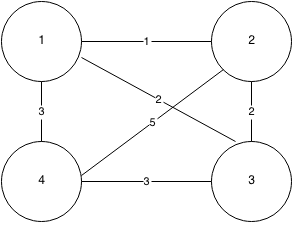
\includegraphics[scale=0.4]{ejemplo_modelado_camiones}
\end{center}

Si resolvemos $k$-PMP en el grafo resultante obtendremos la forma de transportar los productos con tan sólo $k$ camiones
de manera tal que la peligrosidad total sea mínima. Si resolviésemos $k$-PMP en el grafo variando $k$ entre 1 y n
podríamos quedarnos con la primer $k$ que cumpla que cada una de las particiones no supera el umbral de peligrosidad. Sin embargo, no
podemos asegurar que $k$ sea efectivamente la mínima cantidad de camiones. Veamos un ejemplo para ilustrar mejor esto:

\begin{center}
  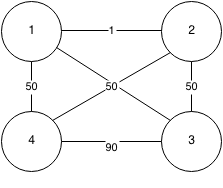
\includegraphics[scale=0.5]{camiones}
\end{center}

Supongamos que el umbral de peligrosidad es $\mu = 50$. Se ve claramente que la partición que devolvería $k$-PMP para $k = 2$ ó $k = 3$ ($k = 1$ y $k = 4$
son únicas por lo cual $k$-PMP y \emph{Biohazard} devolverían la mismo) es $S = \left\{ \left\{1, 2\right\}, \left\{3, 4\right\}\right\}$.
El peso total es $\omega (S) = 1 + 90 = 91$. Por lo tanto, el mínimo $k$ para el cual todas las particiones tienen un peso menor o igual a $\mu$ es
$k = 4$. Sin embargo, tomando $S' = \left\{ \left\{1, 4\right\}, \left\{3, 2\right\}\right\}$ tenemos que $\omega (S) < \omega (S') = 100$
aunque se cumple que $(\forall s'_i \in S' \vert \omega(s'_i) < \mu)$.

Veamos qué pasa si hacemos el camino inverso modelando $k$-PMP como \emph{Biohazard}. Utilizando la misma equivalencia que antes obtenemos
un producto por nodo y la peligrosidad entre dos productos se obtiene como el peso de la arista que une a los nodos correspondientes a esos
productos. Sin embargo, ahora debemos considerar un caso que en primera instancia quedaría afuera del modelo: cuando dos nodos no están unidos 
por ninguna arista en el grafo. Lo que haremos para que nuestro modelo también incluya a este caso será asignarles una peligrosidad igual a 0 
a dos productos cuyos nodos correspondiente no son adyacentes en el grafo. De esta forma podemos asignarles una peligrosidad pero la misma no 
cambia la instancia del problema ya que no aporta peligrosidad. Por último, resta decidir qué umbral de peligrosidad utilizar. En un primer 
momento, parece que el problema no tiene sentido plantearlo como \emph{Biohazard} porque en él buscamos la mínima cantidad de particiones y 
en $k$-PMP ese valor ya lo conocemos, es $k$. Una posibilidad es variar el umbral de peligrosidad de 0 a el peso total del grafo y notar 
los umbrales en los cuales pasa a necesitar un camión más. Podríamos pensar que si necesita $i$ camiones para que niguno supere una peligrosidad
de $\mu$ y precisa $i+1$ para que ninguno supere una peligrosidad de $\mu + 1$ entonces la partición obtenida al utilizar un umbral igual a
$\mu + 1$ se corresponde con la partición de $(i+1)$-PMP. No obstante esto es falso. Un coontraejemplo es la (TODO insertar cita a la figura) FIGURA 2
en la que con $\mu = 49$ necesitamos 3 camiones pero para $\mu = 50$ nos basta con 2 camiones pero la partición correspondiente no es 2-PMP como se
explicó antes.

\subsection{Colores, colores y colores}

Se llama coloreo válido de un grafo a una asignación $f:V \rightarrow C$ tal que:
\begin{displaymath}
f(v) \neq f(u) \quad \forall (u, v) \in E
\end{displaymath}
donde los elementos de $C$ son llamados colores. Además se denomina $k$-coloreo de un grafo $G$ a un coloreo
válido de un grafo que usa exactamente $k$ colores, es decir $\left\vert{C}\right\vert = k$. El problema de coloreo
de un grafo consta de encontrar su coloreo mínimo, un coloreo válido que utilice la mínima cantidad de colores. Podemos
modelar el problema de coloreo de forma tal que si resolvemos $k$-PMP resolvemos coloreo de un grafo.
Sea $G = (V, E)$ el grafo al cual queremos encontrarle el coloreo mínimo. La única transformación que le haremos al grafo 
será asignarle a sus aristas peso 1:
\begin{displaymath}
\omega(v) = 1 \quad \forall v \in V
\end{displaymath}
El procedimiento que realizaremos para obtener el coloreo mínimo de $G$ es resolver $k$-PMP para $k = 1,...,n$ y quedarnos
con el mínimo $k_{min}$ tal que el peso total de la partición es igual a 0:
\begin{displaymath}
  k_{min} = \min_{1 \leq i \leq n} \omega(S_{i-PMP})
\end{displaymath}
con $S_{i-PMP}$ igual a la partición correspondiente a $i$-PMP. Veamos que efectivamente con la partición correspondiente a $k_{min}$-PMP podemos
obtener el coloreo mínimo de $G$. Tenemos que comprobar dos puntos:
\begin{enumerate}
  \item La partición representa un coloreo válido.
  \item El coloreo representado es mínimo.
\end{enumerate}

\paragraph{1)}
Si a cada uno de los $k_{min}$ subconjuntos los pintamos de un color distinto tenemos todo el grafo coloreado
porque todos los nodos pertenecen a algun subconjunto de la partición. Como el peso total de la partición
es igual a 0, $\omega(S_{k_{min}}) = 0$, no puede ser que haya dos nodos adyacentes en la misma partición
porque les habíamos asignado a todas las aristas un peso de 1. Si hubiera dos nodos $u$ y $v$ en una misma
partición tal que $(u, v) \in E$ como $\omega((u,v)) =  1$ y es una arista intrapartición porque estamos
suponiendo que $u$ y $v$ pertenecen a la misma: $\omega(S_{k_{min}}) \geq 1$. Lo cual es absurdo porque 
sabemos que es igual a 0. Por lo tanto, tenemos un coloreo válido porque les asignamos un color a cada nodo 
y nodos con un mismo color no son adyacentes.

\paragraph{2)}
Demostraremos por absurdo que es mínimo. Supongamos que existe un coloreo válido $C$ de $G$ que utiliza $c < k_{min}$ colores.
Si tomamos la partición inducida por el coloreo $C$, es decir tomamos la partición de $V$ que resulta de colocar a los nodos de
colores iguales en el mismo subconjunto, obtenemos una partición con $c < k_{min}$ subconjuntos que tiene un peso total de 0 ya que
los nodos en cada una de las particiones no son adyacentes entre sí. Esto es absurdo porque partimos asumiendo que $k_{min}$ era
la mínima cantidad de subconjuntos necesaria para que el peso total de la partición sea 0.

Así queda demostrado que podemos tomar cualquier grafo $G$ y obtener su coloreo resolviendo $k$-PMP a lo sumo $n$ veces, ya que no
puedo tener una partición con más $n$ subconjuntos, en el grafo obtenido luego de asignarle un peso de 1 a cada una de sus aristas.

Veamos qué sucede si resolvemos coloreo en un grafo para el cual necesitábamos obtener su $k$-PMP. Resulta que el número cromático de 
$G$ $\chi(G)$ se corresponde con $k_{min}$, es decir el mínimo $k$ para el cual el peso total de $k$-PMP es 0. Esto se puede demostrar
con un razonamiento muy parecido al que realizamos para demostrar que el coloreo representado por la partición correspondiente a
$k_{min}$-PMP es mínimio. En primer lugar, construimos la partición correspondiente a algún $\chi(G)$-coloreo ubicando los nodos
de cada color en subconjuntos distintos. Como los nodos de un subconjunto $s_i$ son todos del mismo color y pertenecen a un coloreo válido
entonces no son adyacentes. Por lo tanto, no existen aristas intrapartición. Lo cual implica que el peso total de la partición obtenida
es igual a 0. Desmostramos que es mínimo por absurdo, suponemos:
\begin{displaymath}
  \exists \quad k < \chi(G) \quad | \quad \omega(S_{k}) = 0
\end{displaymath}
pero sabemos que a partir de una partición con peso total igual a 0 podemos obtener un coloreo válido porque las aristas tienen peso 
estrictamente mayor a 0:
\begin{displaymath}
  \omega(e) > 0 \quad \forall e \in E
\end{displaymath}
pero entonces obtendríamos un coloreo válido que utiliza $k < \chi(G)$ colores ya que la cantidad de colores es igual a la cantidad de 
subconjuntos de la partición. Lo cual es absurdo porque por definición $\chi(G)$ es mínimo.
No sólo resolviendo coloreo en un grafo $G$ obtenemos $k_{min}$ y su partición correspondiente, además obtenemos $k$-PMP para todo
$k > k_{min}$ ya que como no podemos obtener un partición con peso estrictamente menor que 0 porque las aristas tiene todas
peso positivo necesariamente la partición correspondiente a $k_{min}$-PMP es mínima para cualquier $k$ mayor. $k_{min}$-PMP
es una partición válida para $k$-PMP con $k > k_{min}$ porque asumimos que tenemos $(k-k_{min})$ subconjuntos vacíos para completar
los $k$ necesarios.

\subsection{$k$-PMP en la vida real}
Como vimos antes $k$-PMP es un problema de optimización combinatoria y cumple con la división de partes definida en el primer punto.
Para cada ejemplo definiremos las partes pertinentes:
\begin{itemize}
  \item \textit{Pabellones de un Hospital}: Se quiere construir un hospital con a lo sumo $k$ pabellones y hay que especializar cada pabellon en áreas de enfermedades lo más compatibles posible. Definimos Las enfermedades como nodos y se analiza un coeficiente de compatibilidad o parentezco entre ellas.

  $X$: Todos los conjuntos k-particiones (se aceptan particiones vacias) son los pabellones en los cuales divido el hospital.

  $P$ e $Y$: Todas las divisiones posibles de menos de $k$ pabellones forman una solución factible.

  $f$: Que la suma de los coeficientes de parentezco entre enfermedades sea mínima.
  \item \textit{Union Deportiva Nacional}: En un país hay que crear a lo sumo $k$ distintas uniones/federaciones de un deporte y quiero que las distancias (aristas) entre las instituciones/entidades (nodos) que conforman la Unión sea mínima.

  $X$: Todos los conjuntos k-particiones (se aceptan particiones vacias) son las Uniones en las cuales divido al pais.

  $P$ e $Y$: Todas las divisiones posibles de menos de $k$ Uniones forman una solución factible.

  $f$: Que la suma de las distancias entre clubes de las uniones sea mínima.
  \item \textit{Impresora}: Una impresora tiene que elegir $k$ colores para imprimir y agrupa los colores más parecidos para usar una tinta de color $k$.

  $X$: Todos los conjuntos k-particiones (se aceptan particiones vacias) son los colores disponibles en la impresora.

  $P$ e $Y$: Todas las divisiones posibles de menos de $k$ colores son una solución posible.
  
  $f$: Que los colores que se imprimen con el mismo color sean lo mas parecidos posibles.
\end{itemize}
